\section{Leaching}
-popis, příčiny a předcházení jevu, význam intermetalických sloučenin v pájeném spoji

\subsection{Zlato}
Zlaté vodiče mají v tlustovrstvých obvodech a strukturách široké uplatnění. Nejčastěji se využívají v aplikacích, u kterých je vyžadovaný vysoký stupeň spolehlivosti jako např. ve vojenských a medicínských aplikacích.

Pokud chceme dosáhnout požadované spolehlivosti, musí být montážní procesy v případě
zlatých vodičů voleny s velkou opatrností (leaching).

Zlato a cín vytváří křehkou intermetalickou sloučeninu s velkým elektrickým odporem.

V případě použití SnPb slitin je třeba použít jako materiál plošek zlato ve slitině s platinou (Pt) nebo paládiem (Pd) - minimalizace leachingu a vzniku nežádoucích intermetalických
sloučenin.

Zlato vytváří intermetalické sloučeniny také s hliníkem (Al), který se využívá pro připojování polovodičových struktur např. pomocí mikrodrátkových propojů (wire bonding -
kontaktování).

Difuzní koeficient hliníku do zlata je mnohem větší než zlata do hliníku - míra difuze rapidně
vzůrstá s teplotou.

Tento jev se může stát významným např. také na rozhraní Au - Al při kontaktování (jak na
čip, tak na TLV plošku). Kdy může např. hliník difundovat do zlatého drátku a přitom za
sebou zanechávat přázdná místa (Kirkendall voids), která oslabují pevnost spoje a zvyšují jeho odpor. Tento jev se výrazně zvyšuje nad teplotou 170 °C a představuje riziko z pohledu
spolehlivosti.

Přídavek paládia do zlata výrazným způsobem snižuje míru difuze a tím zvyšuje spolehlivost
spoje.

\begin{figure}[h]
   \begin{center}
     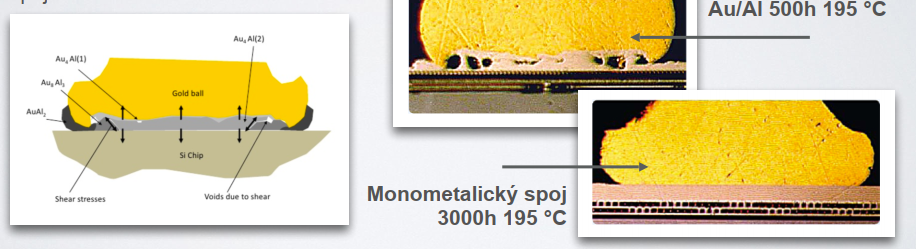
\includegraphics[scale=0.6]{images/Leach.png}
   \end{center}
   \caption{Leaching zlata}
\end{figure}

\subsection{Stříbro}
Stříbro je nejčastěji používáno v komerčních aplikacích, kde je výsledná cena důležitým faktorem. Stejně tak jako zlato je i stříbro náchylné k leachingu do SnPb pájek, ovšem s menší intenzitou. Minimalizovat tento efekt je možné pomocí niklu naneseného na povrch pájecí plošky.

Stříbro má tendenci navíc k elektromigraci v případě, kdy se mezi dvěma vodiči vyskytuje elektrický potenciál (za současné přítomnosti tekuté vody).

Tento jev se vyskytuje i u jiných materiálů (Au, Pb, Sn, …), Ag je tento jev výrazně
významnější díky svému velkému ionizačnímu potenciálu.

\begin{figure}[h]
   \begin{center}
     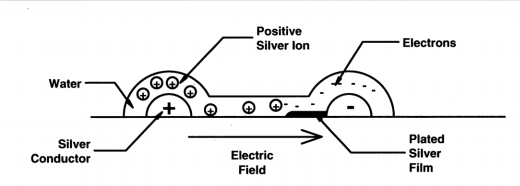
\includegraphics[scale=0.6]{images/Migrace.png}
   \end{center}
   \caption{Elektromigrace}
\end{figure}

\subsection{Význam intermetalických sloučenin v pájeném spoji}
Slitiny stříbra s paládiem a/nebo platinou vykazují jak snížení náchylnosti k leachingu, tak
náchylnosti k elektromigraci, což je předurčuje k využití v případě potřeby pájet.

Pd/Ag vodivé pasty jsou nejběžněji používané materiály v komerční oblasti TLV a hybridních
integrovaných obvodů.

Je třeba si však uvědomit, že přídavek paládia navyšuje jak cenu pasty, tak její výsledný
elektrický odpor.

Nejčastěji je proto používán poměr 4 díly Ag ku 1 dílu Pd, což poskytuje dobrý kompromis mezi
parametry pasty a její cenou.


















